\section{Metodologia}

\subsection{Descrição do Sistema e Modelagem matemática}

O sistema utilizado neste trabalho, conforme descrito por \citet{wildson_2024}, é composto por dois tanques esféricos interligados, como mostrado na Figura \ref{fig:tank-system}. Ambos sujeitos à pressão atmosférica. A dinâmica do sistema inclui uma entrada de fluido para o tanque 1 e uma saída de fluido do tanque 2, cuja vazão depende diretamente do nível do líquido no segundo tanque. Para simplificar as equações, assume-se que o líquido é incompressível e possui massa específica constante.

\begin{figure}[ht]
  \centering
  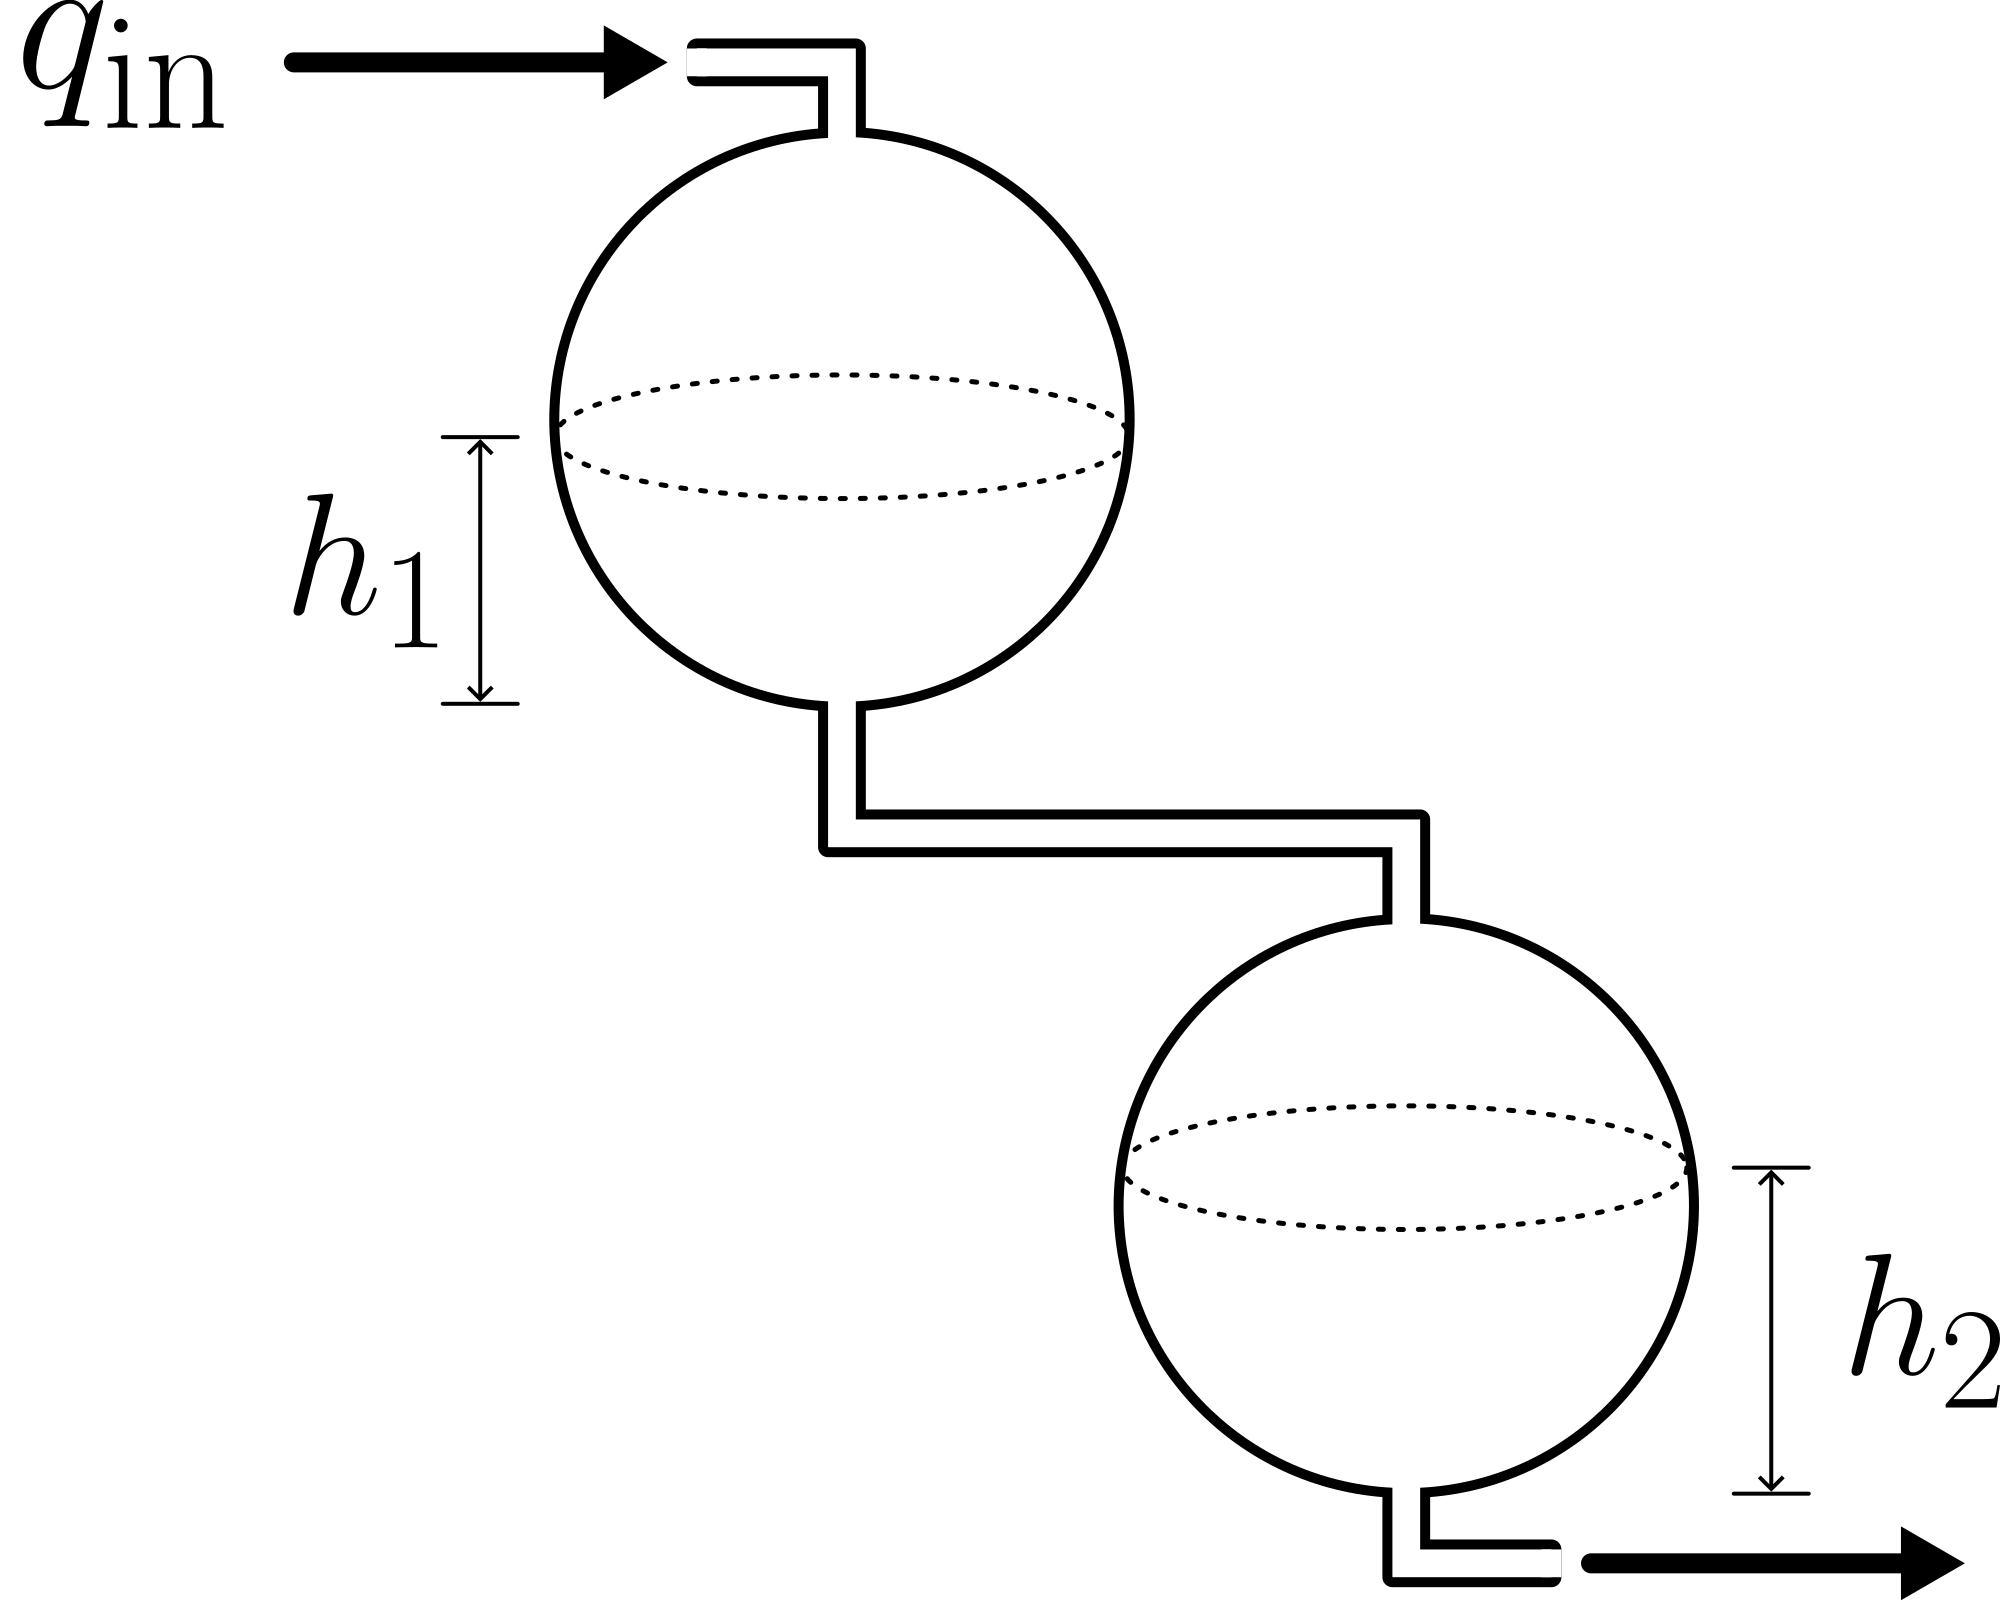
\includegraphics[width=0.3\textwidth]{tank-system.png}
  \caption{Representação esquemática do sistema de dois tanques esféricos.}
  \label{fig:tank-system}
\end{figure}

A modelagem baseia-se no princípio de conservação de massa, onde a taxa de variação do volume de líquido em cada tanque é dada pela diferença entre a vazão de entrada $q_{\mathrm{in}}$ e de saída $q_{\mathrm{out}}$, conforme a equação:
\begin{equation}
  \diff{V(t)}{t}=q_{\mathrm{in}}-q_{\mathrm{out}}
  \label{eq:conservation_of_mass}
\end{equation}

Para expressar a equação \ref{eq:conservation_of_mass} em termos de nível de líquido, é necessário dividir ambos os lados pela área da seção transversal do tanque, que, no caso de um tanque esférico, é uma função não linear da altura do líquido.

Como o sistema trata de dois tanques interligados, a vazão de saída do tanque 1 torna-se a vazão de entrada do tanque 2. Assim, a dinâmica de um tanque afeta diretamente o outro. Com isso, obtemos o sistema de equações diferenciais:

\begin{equation}
  \begin{cases}
    \displaystyle \diff{h_1(t)}{t} & =
    \displaystyle \frac{
      q_{\mathrm{in}} - \alpha_1 s_1 \sqrt{2gh_1}
    }{
      \pi (2 R h_1 - h_1 \, ^2)
    } %
    \\[10pt]
    \displaystyle \diff{h_2(t)}{t} & = %
    \displaystyle \frac{
      \alpha_1 s_1 \sqrt{2gh_1} - \alpha_2 s_2 \sqrt{2gh_2}
    }{
      \pi (2 R h_2 - h_2 \, ^2)
    }
  \end{cases}
  \label{eq:tank_system}
\end{equation}%
que descrevem a variação temporal do nível de líquido em cada tanque.

O valor e o significado de cada um dos parâmetros e constantes utilizados na modelagem, como área da seção transversal da tubulação e coeficientes relacionados à geometria dos tanques, são descritos com seus valores na Tabela \ref{tab:tanks_params}.

\begin{table}[ht]
  \centering
  \caption{Constantes do sistema de equações~\ref{eq:tank_system}.}
  \label{tab:tanks_params}
  \begin{tabular}{ccc}
    Símbolo    & Descrição                          & Valor               \\ \hline
    $\alpha_1$ & Fator de correção 1                & $0.56$              \\
    $\alpha_2$ & Fator de correção 2                & $0.30$              \\
    $s_1$      & Área da seção de saída do tanque 1 & $0.50 \, cm^2$      \\
    $s_2$      & Área da seção de saída do tanque 2 & $0.50 \, cm^2$      \\
    $g$        & Aceleração da gravidade            & $980.665 \, cm/s^2$ \\
    $R$        & Raio dos tanques                   & $14.85 \, cm$       \\ \hline
  \end{tabular}
\end{table}

\subsection{Desenvolvimento e Estrutura da Rede Neural}

As ANNs são modelos computacionais inspirados no funcionamento do cérebro humano. Elas consistem em camadas compostas de neurônios artificiais, elementos de processamento capazes de receber entradas e produzir uma saída com base em funções matemáticas. Cada neurônio realiza operações simples sobre suas entradas e as transmite para os neurônios da camada seguinte, permitindo a construção de representações mais complexas à medida que os dados passam pelas camadas da rede neural \citep{mu_sun_2022}. Elas são amplamente utilizadas na indústria química por sua capacidade de processar dados complexos e não-lineares comuns a essa indústria, tudo isso sendo consideradas modelos do tipo ``caixa preta'', onde as relações matemáticas entre variáveis não precisam ser conhecidas de antemão. Isso é especialmente útil quando não se tem um bom modelo matemático para o sistema, por ser possível construir modelos baseados unicamente em dados \citep{wang_2022}.

Entretanto, os modelos puramente baseados em dados apresentam limitações consideráveis. Para que esses modelos sejam eficazes, eles demandam um grande volume de dados representativos e abrangentes, algo nem sempre viável. Além disso, eles carecem de capacidade para extrapolar além das condições observadas nos dados de treinamento. Outro ponto crítico é que esses modelos podem gerar previsões inconsistentes com o conhecimento científico existente, pois não consideram as leis físicas que governam o sistema \citep{karniadakis_2021}. Então, para superar essas limitações e aproveitar o conhecimento físico disponível, surgiram as PINNs, introduzidas por \citeauthor{raissi_2017_I} em \citeyear{raissi_2017_I}. Elas Funcionam de forma parecida com às redes neurais artificiais tradicionais, com a diferença de que, além do custo associado aos dados, a função de custo também considera o erro relacionado ao problema físico, ou seja, a rede neural é penalizada ao diferir das relações físicas já conhecidas.

Da mesma maneira, as PIRNNs foram propostas como uma extensão das PINNs, combinando sua capacidade de incorporar conhecimento físico com a habilidade das redes neurais recorrentes (\textit{Recurrent Neural Networks} — RNNs) de processar dados sequenciais e capturar dependências temporais eficientemente \citep{zheng_2023}.

No caso da PIRNN utilizada neste trabalho, as entradas são compostas por dois valores anteriores dos estados do sistema ($h_1$, $h_2$) e da vazão de entrada $q_{\mathrm{in}}$, enquanto a saída da rede corresponde aos próximos valores dos níveis dos tanques. Dependendo da aplicação, a entrada pode ser composta por um valor anterior e um atual ($t{-}1$ e $t$) para a rede retornar o valor futuro ($t{+}1$), ou, como foi utilizado neste trabalho, dois pontos anteriores ($t{-}2$ e $t{-}1$) para retornar o valor presente ($t$). A arquitetura da rede é composta por uma camada recorrente do tipo \textit{Elman} \citep{elman_1990} seguida por camadas lineares totalmente conectadas. Para treiná-la, a função de custo adotada é composta pela soma do custo associado as equações diferenciais ($L_{\mathrm{EDOs}}$) e o custo relacionado aos dados de treinamento ($L_{\mathrm{data}}$). Os dados utilizados foram obtidos por meio de simulações computacionais com métodos numéricos tradicionais, uma vez que a física do problema está bem definida e permite gerar dados confiáveis para a modelagem. No total, a função de custo é definida como:
\begin{equation}
  L = \omega_1 \cdot L_{\mathrm{EDOs}} + \omega_2 \cdot L_{\mathrm{data}},
\end{equation}
onde
\begin{equation}
  \begin{aligned}
    L_{\mathrm{EDOs}} & = \frac{1}{N} \sum_{i=1}^{N} ( \diff{y_{\mathrm{prev},i}}{t} - f(y_{\mathrm{prev},i}))^2 \\
    L_{\mathrm{data}} & = \frac{1}{N} \sum_{i=1}^{N} (y_{\mathrm{data},i} - y_{\mathrm{prev},i})^2
  \end{aligned}
\end{equation}
Sendo os pesos $\omega_1$ e $\omega_2$ coeficientes ajustáveis que determinam a importância relativa de cada termo na função de custo, $y_{\mathrm{data}}$ os dados obtidos pela simulação, $y_{\mathrm{prev}}$ os valores de saída previstos pela rede neural e $f$ o sistema de equações diferencias \ref{eq:tank_system}. A derivada em relação ao tempo foi calculada por meio do método das diferenças finitas com 3 pontos, considerando os dois pontos fornecidos para a rede e o ponto previsto pela rede.

O treinamento da rede foi realizado utilizando o otimizador \textit{Adam} no framework PyTorch \citep{kingma_2017, pytorch_2024}. Para otimizar a inferência em tempo de execução, o modelo treinado foi convertido para o formato ONNX (\textit{Open Neural Network Exchange}), e os testes de velocidade foram realizados com o framework \textit{ONNX Runtime} \citep{onnxruntime}.

\subsection{Implementação no Arduino}

Criado em 2005, o Arduino é uma plataforma prototipagem amplamente utilizada por programadores devido ao seu baixo custo e facilidade para desenvolver. A plataforma conta com uma série de placas diferentes, cada uma com características específicas, para atender a diversas necessidades e aplicações. Entre as placas mais populares, destaca-se o Arduino UNO, uma das primeiras e mais acessíveis opções disponíveis e que foi a escolhida para esse trabalho \citep{hughes_2016}.

No entanto, o Arduino é bem limitado em termos de capacidade de memória e processamento. O modelo UNO, possui 32 kilobytes de memória flash e apenas 2 kilobytes de memória RAM, o que dificulta bastante a tarefa de implementar algoritmos mais complexos, como redes neurais que possuem muitas camadas. Nesse trabalho, para garantir que o código fosse compatível com as restrições do hardware, foram feitas otimizações para reduzir o uso de memória e armazenamento. Dentre elas, vale a pena destacar o uso da memória flash para armazenamento dos pesos e bias da rede neural por meio da diretiva \textit{PROGMEM} \citep{margolis_2020}. Isso é possível, pois esses valores são constantes, uma vez que foram definidos na etapa de treinamento da rede.

% Pequena gambiarra aqui. Essas duas figuras tiveram que mudar de posição para ajuste de layout.
\begin{figure}[ht]
  \centering
  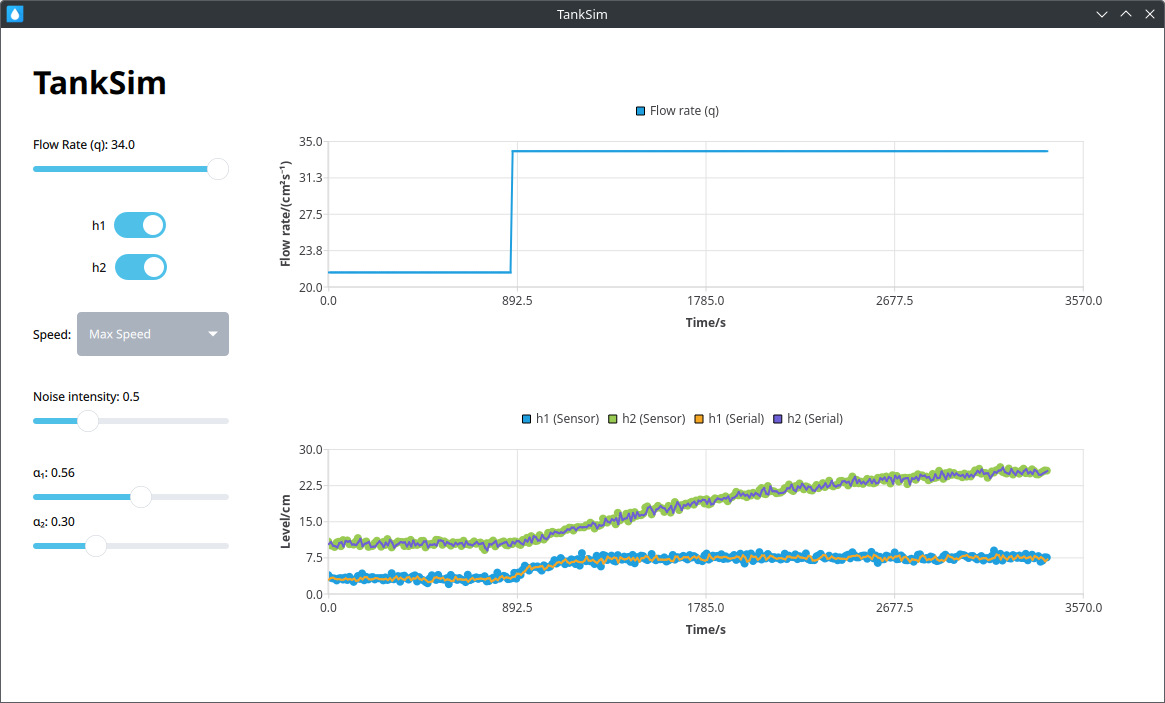
\includegraphics[width=0.4\textwidth]{tanksim.png}
  \caption{Captura de tela do TankSim.}
  \label{fig:interface}
\end{figure}

\begin{figure*}[ht]
  \centering
  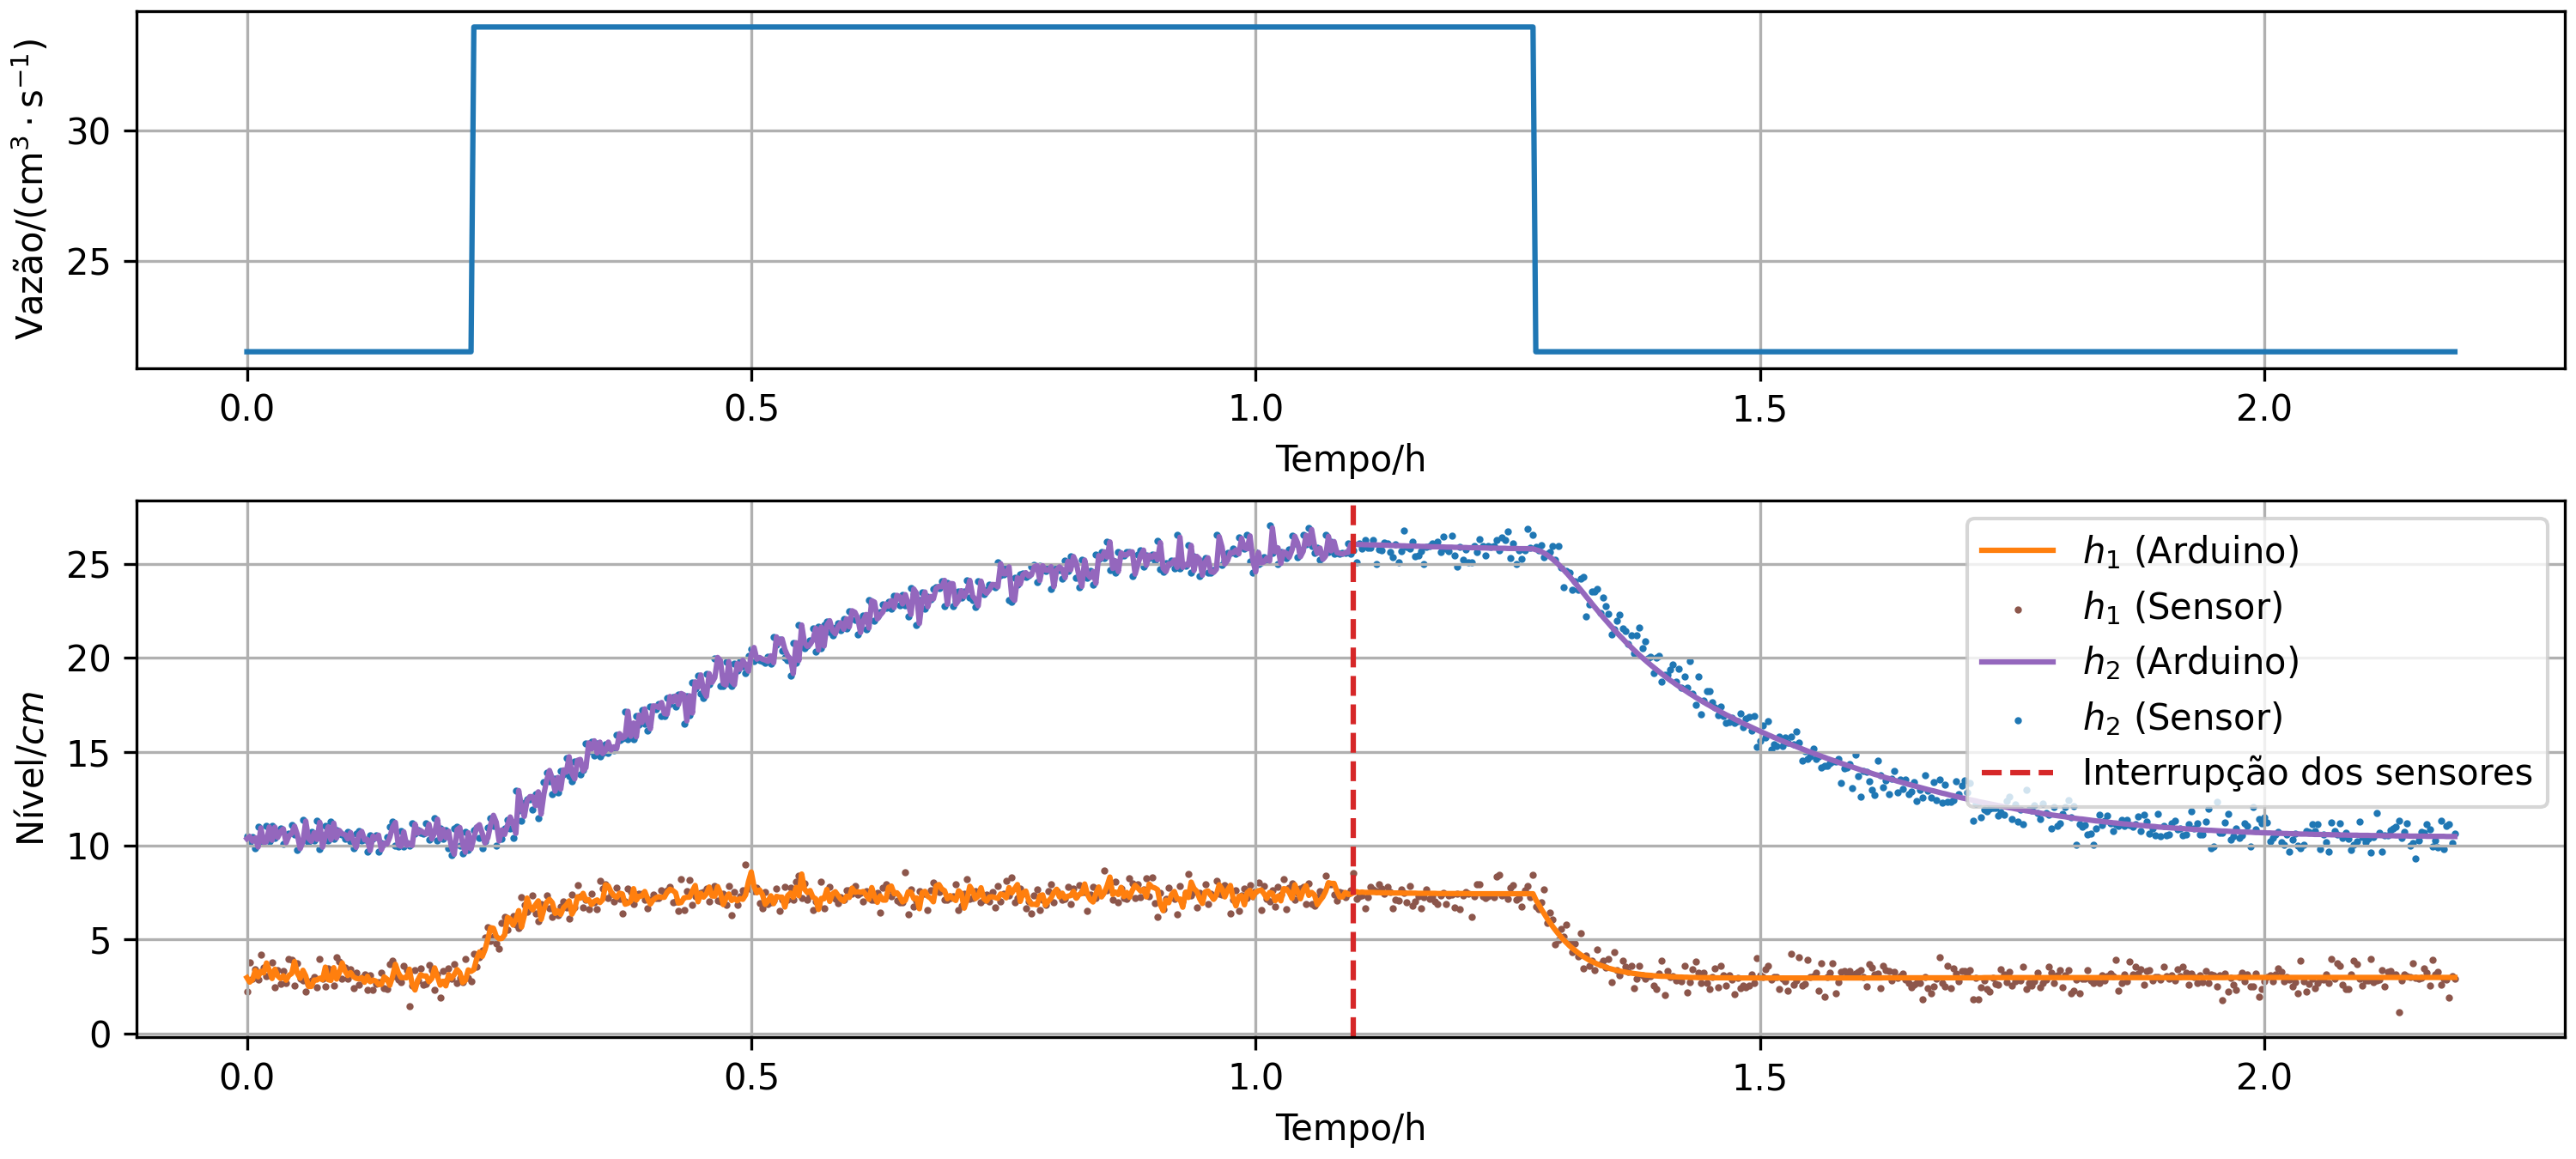
\includegraphics[width=0.8\textwidth]{sil-pirnn.png}
  \caption{Comparação entre as leituras dos sensores, obtidas a partir dos níveis simulados com adição de ruído, e os níveis previstos pela PIRNN embarcada após uma perturbação do tipo degrau na vazão de entrada. A linha tracejada vermelha vertical indica o instante em que os valores dos sensores deixam de ser enviados ao Arduino, fazendo com que a PIRNN passe a se retroalimentar.}
  \label{fig:sil-pirnn}
\end{figure*}

Para realizar a comunicação com o Arduíno, foi desenvolvido o \textit{software} \textit{TankSim} (Figura \ref{fig:interface}), responsável por simular o funcionamento do sistema, enviar os dados simulados para o Arduino e receber os valores previstos pela rede neural, além de plotar os gráficos comparando os dados simulados com os previstos. A interface conta ainda com um controle deslizante que permite o usuário alterar a vazão de entrada $q_{\mathrm{in}}$, dois interruptores para suspender o envio dos dados simulados do nível dos tanques para o Arduino e outro controle deslizante para controlar o nível de ruído. A interface foi programada utilizando o framework \texttt{Qt} (\url{https://www.qt.io/}), que oferece uma ampla gama de componentes e ferramentas para a criação de interfaces.

%alterar os valores de $\alpha_1$ e $\alpha_2$ (visando simular a degradação do modelo frente a uma mudança nos parâmetros dos tanques)

% Local original da figura fig:interface

No total, este sistema configura-se como um esquema \textit{software-in-the-loop} (SIL) \citep{chen_2008}. Nele, o \textit{TankSim} simula o envio de dados dos sensores de uma planta para o Arduino, que, por sua vez, responde com os dados previstos pela rede neural, ou seja, os prováveis valores para o nível de líquido em cada tanque no próximo intervalo de tempo. Quando os dados dos sensores não estão disponíveis, simulando uma falha ou interrupção manual por meio dos interruptores da interface, o Arduino entra em um modo de retroalimentação. Nesse modo, ele utiliza os valores previstos pela rede neural como entrada para gerar a previsão do próximo valor, mantendo a operação do sistema mesmo com os sensores indisponíveis.
